% Fig.3: source PDF 2018春季上海 p4. Schematic spatial view; no projected lengths imply actual metric lengths.
% C is the base centre; AB, DE are base diameters; O is midpoint of SE; OC || SD.
% The section is the parabola P(t)=O*(1-t^2)+A*t after projection; hidden branch A--O is dashed.
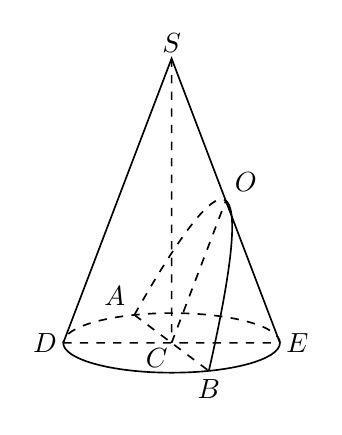
\begin{tikzpicture}[x=.86cm,y=.86cm,line width=.6pt,font=\normalsize]
\coordinate (S) at (0,4.2);\coordinate (C) at (0,0);
\coordinate (D) at (-1.6,0);\coordinate (E) at (1.6,0);
\coordinate (A) at (-.55,.41319);\coordinate (B) at (.55,-.41319);
\coordinate (O) at (.8,2.1);
\draw (D)--(S)--(E);
\draw (D) arc[start angle=180,end angle=360,x radius=1.6,y radius=.44];
\draw[dashed] (E) arc[start angle=0,end angle=180,x radius=1.6,y radius=.44];
\draw[dashed] (D)--(E) (A)--(B) (S)--(C) (C)--(O);
\draw[dashed] plot[domain=1:0,samples=45] ({.8*(1-\x*\x)-.55*\x},{2.1*(1-\x*\x)+.41319*\x});
\draw plot[domain=0:-1,samples=45] ({.8*(1-\x*\x)-.55*\x},{2.1*(1-\x*\x)+.41319*\x});
\node[above,inner sep=2pt] at (S) {$S$};
\node[left,inner sep=2pt] at (D) {$D$};
\node[right,inner sep=2pt] at (E) {$E$};
\node[above left,inner sep=3pt] at (A) {$A$};
\node[below,inner sep=3pt] at (B) {$B$};
\node[inner sep=0pt] at (-.22,-.22) {$C$};
\node[above right,inner sep=3pt] at (O) {$O$};
\end{tikzpicture}
